\chapter{艇员管理系统}
A crew management system can store the training record and provide a great feed
back for the training crew. Our crew is training on a daily basis, one finds
that by comparing and contrast, would make a positive and huge impact on the
confidence and momentum of he training individuals as well as crew members.
In the old school ways, our crew members have to use pen and paper to write down
their training results, and later need to be typed into computers. Therefore
developing a crew management system would greatly enhance the efficiency in
terms of designing training plans and logging training results
.
艇员管理系统是一个能够发布训练计划,统计训练记录的系统。并能通过统计得到的训练记
录进行反馈,为队员提供参考。一个体育团队通过收集每天的训练情况来定期给队员提供积
极科学的反馈,并以此能够修正训练计划,从而使训练更加高效有序。可是现实团队里面在
即时通讯软件(wechat)里面发布和收集训练记录,或者说用纸来记录数据。这样的做法费
时费力而且数据也不完整,即使通信软件里面有相当强大的搜索功能。但是如果每次进行数
据收集都是对聊天记录进行搜索的话,数据难免丢失(数据格式不一致等原因)因此开发一
个数据库应用来进行队内事务管理是相当有必要的。

\newpage

\section{开发环境与开发工具}

\section{系统需求分析}% need further investigation, query somebody maybe
% \begin{enumerate}
% \item
%   {system user management
%     \begin{enumerate}
%     \item{user adding\\
%         include 3 kinds of member type: Crew Coach, Crew Leader, Crew member\\
        
%         Crew Coach can announce the plans for this year: have access to
%         modifying the calender: dates for group extra training program, dates for out
%         field races, etc..\\
        
%         Crew Leader can design and publish training plans(in the form of
%         notice-board) and specify the training program for the day. Have access
%         to team budgets, logging of team budgets.\\
        
%         Crew members can update their status on the training program of the day.
%         How many push-ups and squats(training programs of the day), how much time
%         for the 10 laps running, etc..\\

%         Crew member information: Entrance date, height, weight, age.
        
%         To be continued...
%         }
%       \item{user deletion\\
%           the deletion of the mentioned crew member types. Cascade deletion(deleting
%           team members would also delete their training records)
%         }
%       \item{password modification
%           add password, update password. Involves registration.\\
%         }
%     \end{enumerate}
%   }

% \item{training plans management\\
%     training plans CRUD(Create, Read, Update, Delete):
%   }

% \item {
%     training log management\\
%     training log CRUD
%   }

% \item {
%     Crew members information management\\
%     crew members information CRUD
%   }

% \item {
    
%   }
  
% \end{enumerate}

\begin{enumerate}
\item
  {系统的用户管理\\
    包括用户的添加、删除、修改信息、修改密码等。

    一个用户对应一个成员,有唯一的用户名作为标识符,需要密码进行登录。
  }

\item{艇员信息管理\\
    艇员信息的添加、删除、修改、查询。

    一个成员有自己的各种信息,对应唯一一个账户,有自己的训练级别,还有多条自己的
    训练记录,有多条对应自己的开支,由(ID)唯一标识。
    
  }

\item{训练计划管理\\
    训练计划的添加,修改,删除,查询。

    一个训练计划包含训练时间,训练时长,训练项目,训练指标,还有训练对应的级别,
    由(plan\_ID)唯一标识,需要和成员联系,作为计划制定者。
  }

\item {训练记录管理\\
    训练记录的添加,修改,删除,查询。

    一个训练记录(与训练计划对称),有训练时间,训练时长,训练项目,训练结果,由
    (record\_ID)唯一标识,需要和成员联系,作为训练者。
    
  }

\item {船艇信息\\
    艇的信息添加,修改,删除,查询。

    一艘艇有名字,有类型,由(ship\_ID)唯一标识。
  }

\item {开支信息\\
    开支记录的添加,修改,删除,查询。

    一条开支,有时间,有备注,需要和成员联系,作为支出的对象,由(fee\_ID)唯一标
    识。
  }

\end{enumerate}





%making the blow text smaller perhaps?

\section{功能需求分析}
艇员管理系统按照上面所述,管理功能主要在艇员信息、训练计划和训练记录的管理上面。
下面还有一些主要的功能说明
\begin{enumerate}
\item{其中用户分为两个级别。普通用户级别和特权用户级别。特权用户级别的操作是普通用户级别的超集。}

\item{其中添加、删除操作输入特权用户级别,AKA只有特权用户能够添加新的成员。而每个用户需要自己的艇员信息被录入才能注册新的用户。每个用户能够对自己的信息进行查询,对部分信息能够进行修改。}

\item{其中添加,修改,删除属于特权用户级别。}

\item{每个用户只能对自己的训练记录进行(CUD--Create, Update, Delete)。每个用户可以查询其他用户的训练记录。}

\item{普通用户只能部分修改,能够查询。}
\end{enumerate}

\section{系统设计}
\subsection{系统ER图}

% \usetikzlibrary{shapes.geometric, arrows, decorations.markings}
\usetikzlibrary{arrows,decorations.pathmorphing,backgrounds,positioning,fit,petri,
shapes.geometric, decorations.markings}

\tikzstyle{vecArrow} = [thick, decoration={markings,mark=at position
   1 with {\arrow[semithick]{open triangle 60}}},
   double distance=1.4pt, shorten >= 5.5pt,
   preaction = {decorate},
   postaction = {draw,line width=1.4pt, white,shorten >= 4.5pt}]

\tikzstyle{entity} = [rectangle, minimum width=3cm, minimum height=1cm,
                      text width=3cm,
                      fill=white,
                      draw=black,
                      text centered,
                      top color=gray,
                      opacity=0.5,
                      bottom color=white]
                      
\tikzstyle{relationship} = [diamond, minimum width=3cm, minimum height=1cm,
                      text width=3cm,
                      fill=white,
                      draw=black]

\tikzstyle{attribute} = [rectangle, minimum width=3cm, minimum height=1cm,
                      text width=3cm,
                      fill=white,
                      draw=black]
                      

% \tikzstyle{attribute} = [top color=white, bottom color=yellow!20, 
%                                draw=yellow, node distance=1cm]
\tikzstyle{isa} = [top color=white, bottom color=green!20, 
                         draw=green!50!black!100]


\centering
\scalebox{.5}{
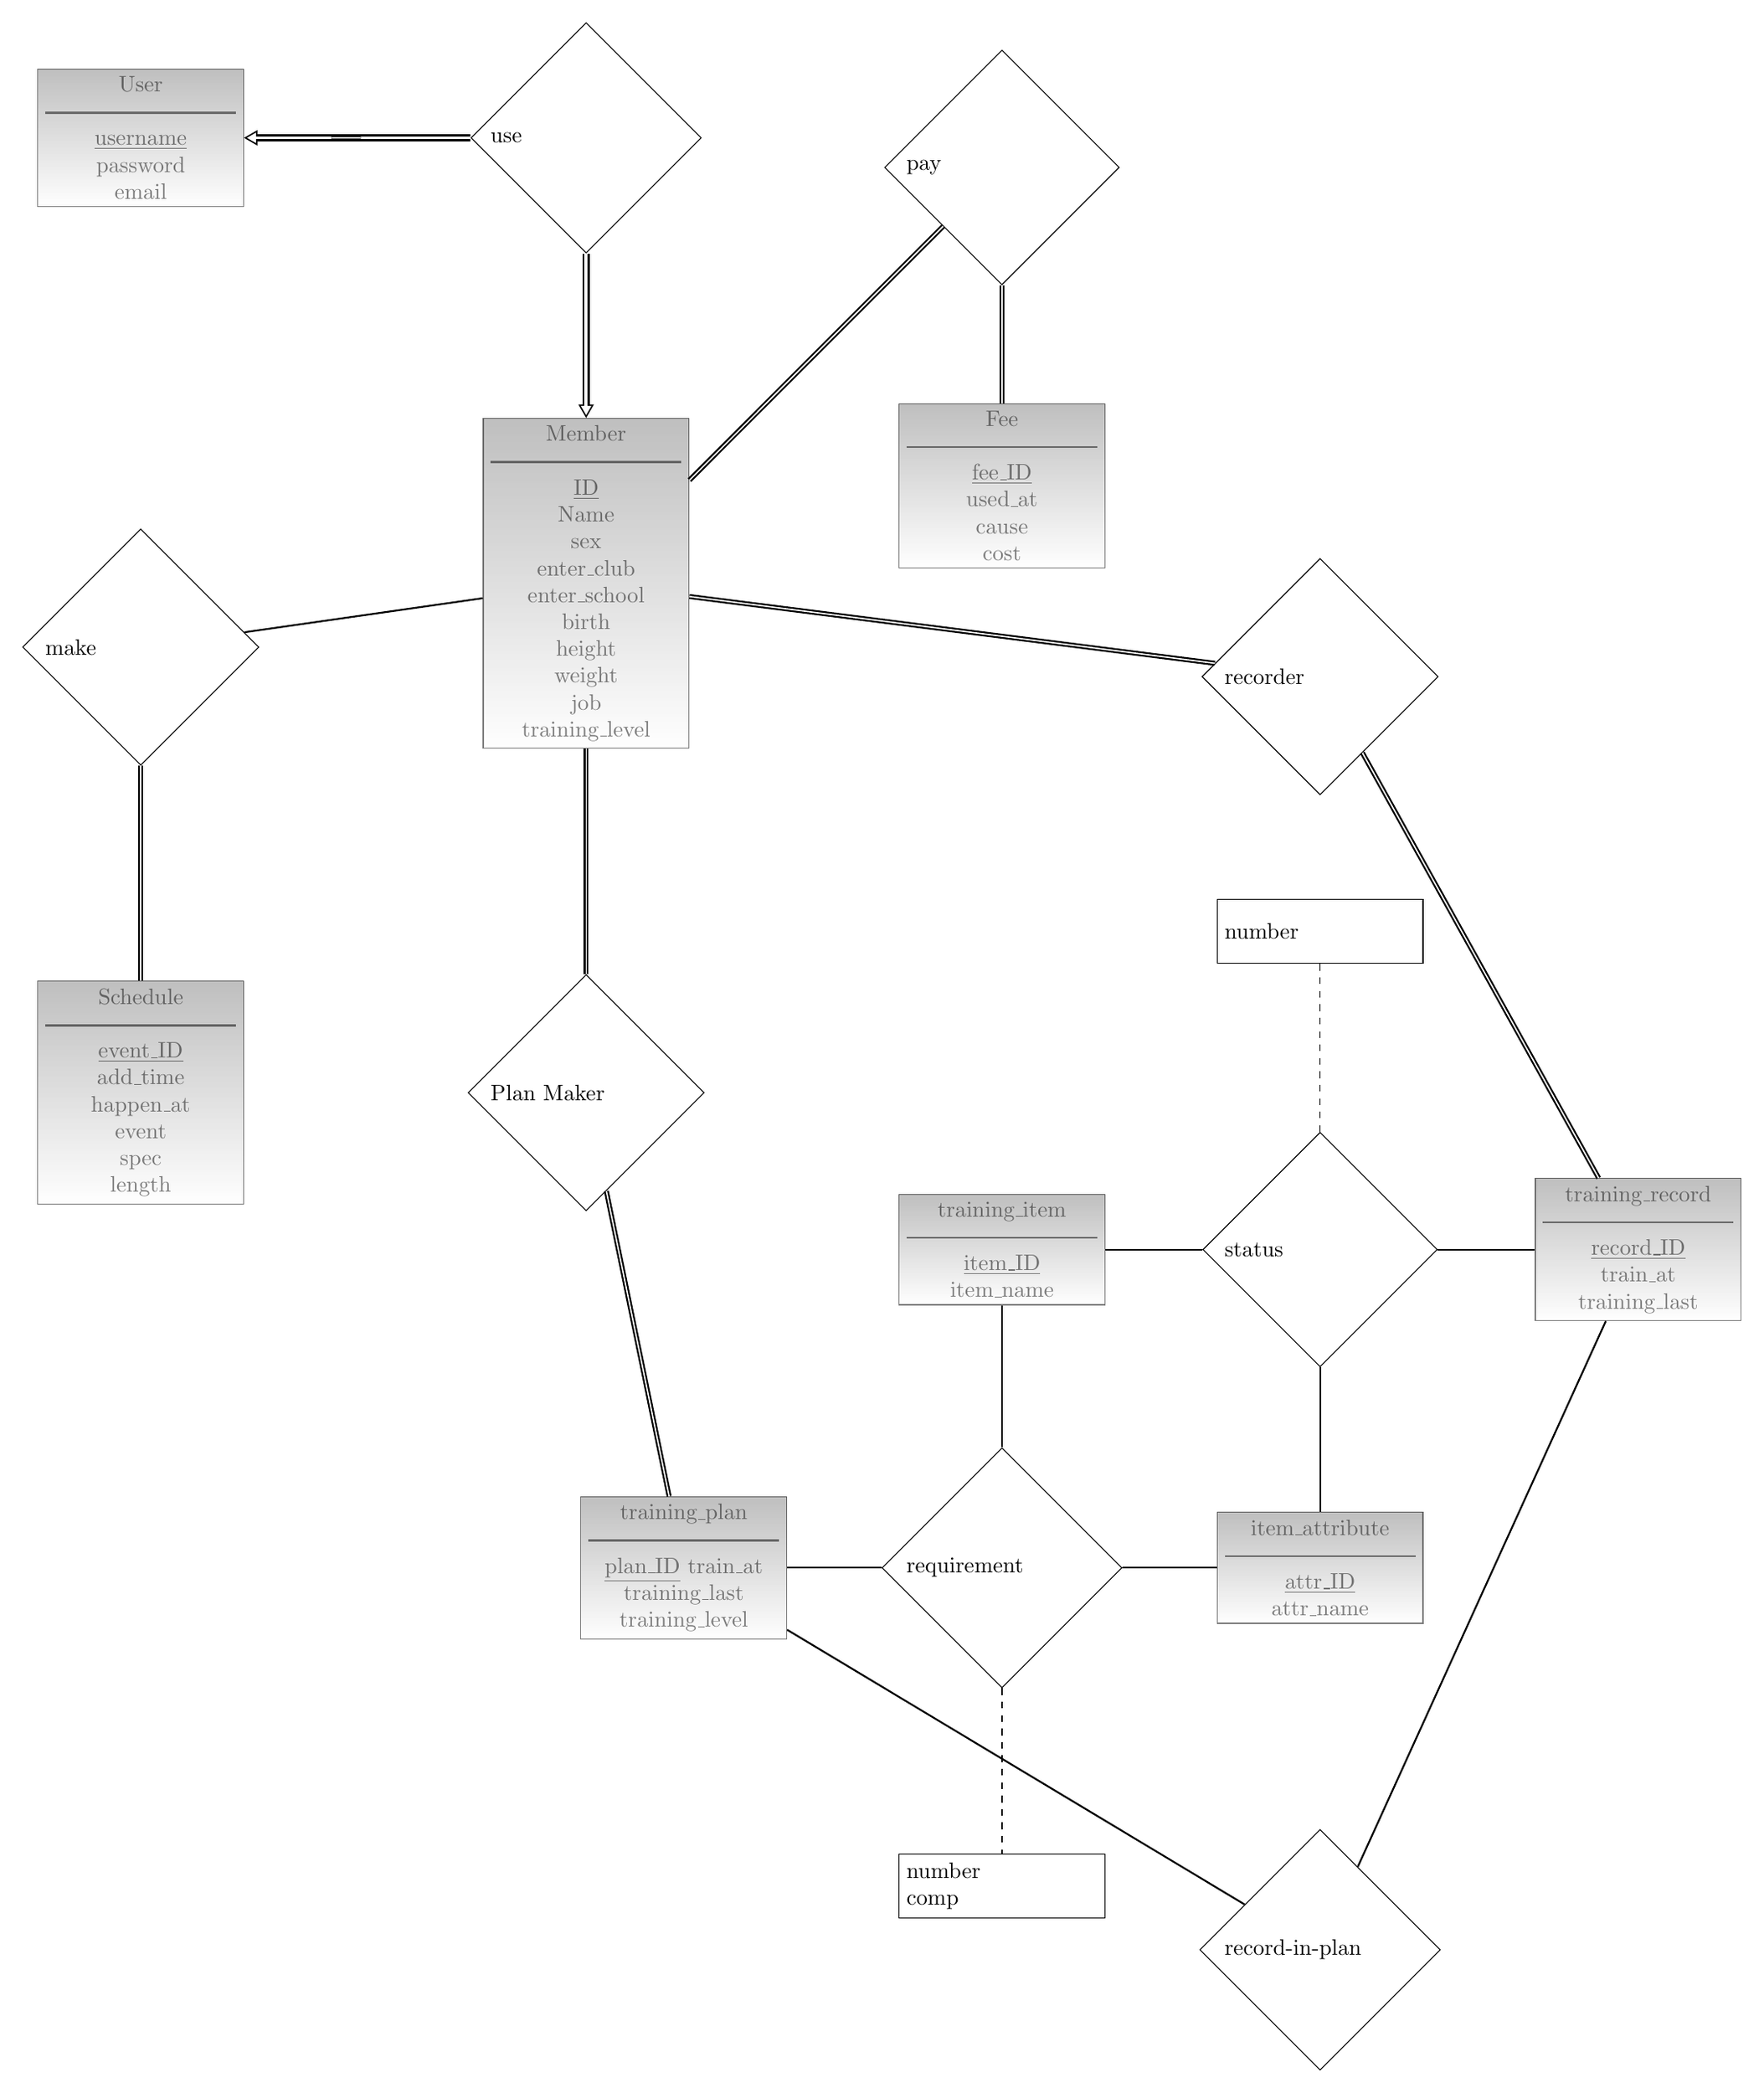
\begin{tikzpicture}[node distance=5cm]

  \node (user) [entity, xshift=-3cm] {
    User\\
    \noindent\rule[0.5ex]{3cm}{1pt}
    
    \underline{username}\\
    password\\
    email\\
  };

  \node (use) [relationship, right of=user, xshift=2cm] {
    use
  };

  \node (member) [entity, below of=use, yshift=-2cm] {
    Member \\
    \noindent\rule[0.5ex]{3cm}{1pt}

    \underline{ID}\\
    Name\\
    sex\\
    enter\_club\\
    enter\_school\\
    birth\\
    height\\
    weight\\
    job\\
    training\_level\\
  };

  \draw[vecArrow] (use) to (user);
  \draw[vecArrow] (use) to (member);

  %   \draw[thick, double](0,0)--(3ex,0) (use) to (user);
  % \draw[thick, double](0,0)--(3ex,0) (use) to (member);


  \node (schedule) [entity, below of=user, yshift=-10cm] {
    Schedule\\
    \noindent\rule[0.5ex]{3cm}{1pt}

    \underline{event\_ID}\\
    add\_time\\
    happen\_at\\
    event\\
    spec\\
    length\\
  };

  \node (make) [relationship, below of=user, yshift=-3cm] {
    make
  };

  \draw[thick, double](0,0)--(3ex,0) (make) to (schedule);
  \draw[thick] (make) to (member);

  \node(pay) [relationship, above right of=member, xshift=3cm, yshift=3cm] {
    pay
  };

  \node (fee) [entity, below of=pay] {
    Fee\\
    \noindent\rule[0.5ex]{3cm}{1pt}

    \underline{fee\_ID}\\
    used\_at\\
    cause\\
    cost\\
  };


  \draw[thick, double](0,0)--(3ex,0) (pay) to (fee);
  \draw[thick, double](0,0)--(3ex,0) (pay) to (member);

  \node (item) [entity, below of=fee, yshift=-7cm] {
    training\_item\\
    \noindent\rule[0.5ex]{3cm}{1pt}
    
    \underline{item\_ID}\\
    item\_name\\
  };

  \node(requirement) [relationship, below of=item] {
    requirement
  };

  \node(status) [relationship, right of=item] {
    status
  };

  \node(req-attr) [attribute, below of=requirement] {
    number\\
    comp
  };

  \node(sta-attr) [attribute, above of=status] {
    number\\
  };

  \node (record) [entity, right of=status] {
    training\_record\\
    \noindent\rule[0.5ex]{3cm}{1pt}

    \underline{record\_ID}\\
    train\_at\\
    training\_last\\
  };

  \node (plan) [entity, left of=requirement] {
    training\_plan\\
    \noindent\rule[0.5ex]{3cm}{1pt}
    
    \underline{plan\_ID}
    train\_at\\
    training\_last\\
    training\_level\\ % take note here, need changes
  };

  \node (attribute) [entity, right of=requirement] {
    item\_attribute\\
    \noindent\rule[0.5ex]{3cm}{1pt}

    \underline{attr\_ID}\\
    attr\_name\\
  };

  \draw[thick] (requirement) to (plan);
  \draw[thick] (requirement) to (item);
  \draw[thick] (requirement) to (attribute);

  \draw[thick] (status) to (item);
  \draw[thick] (status) to (attribute);
  \draw[thick] (status) to (record);
  
  \draw[dashed] (requirement) to (req-attr);
  \draw[dashed] (status) to (sta-attr);

  \node(plan-maker) [relationship, below of=member, yshift=-3cm] {
    Plan Maker
  };

  \node(recorder) [relationship, right of=fee, yshift=-3cm] {
    recorder
  };

  \draw[thick, double](0,0)--(3ex,0) (plan-maker) to (plan);
  \draw[thick, double](0,0)--(3ex,0) (plan-maker) to (member);

  \draw[thick, double](0,0)--(3ex,0) (recorder) to (record);
  \draw[thick, double](0,0)--(3ex,0) (recorder) to (member);
  
  \node(record-in-plan) [relationship, below of=attribute, yshift=-1cm] {
    record-in-plan
  };

  \draw[thick] (record-in-plan) to (record);
  \draw[thick] (record-in-plan) to (plan);

  % \node(ship) [entity] {
  %   ship\\
  %   \noindent\rule[0.5ex]{3cm}{1pt}
    
  %   \underline{name}\\
  %   condition\\
  % };

  % \node(ship type) [entity, right of=ship] {
  %   ship\_type\\
  %   \noindent\rule[0.5ex]{3cm}{1pt}

  %   type\_ID\\
  %   ship\_type\_name\\
  % };
      
\end{tikzpicture}
}
\subsection{数据流程图}

图中的系统层就是我们设计的网页应用。他简化了用户和数据库的交互,并提供一定的等级
分层,以及维护系统的数据完整性。

\begin{tikzpicture}
  [node distance=3cm,
  module/.style={circle, draw=blue!50, fill=blue!20,
    thick, inner sep=0pt, minimum size=2cm},
  manage/.style={rectangle, draw=blue!50, fill=blue!20,
    thick, inner sep=0pt, minimum size=1cm}]
  
  \node[module] (user)                           {用户};
  \node[module] (system) [right=of user]         {系统};
  
  \node[manage] (account) [above right=of system, yshift=1cm, xshift=2cm] {账号信息管理};
  \node[manage] (member) [below =of account, yshift=2cm] {成员信息管理};
  \node[manage] (fee) [below =of member, yshift=2cm] {开支信息管理};
  \node[manage] (ship) [below =of fee, yshift=2cm] {艇支信息管理};
  \node[manage] (training-plan) [below =of ship, yshift=2cm] {训练计划管理};
  \node[manage] (training-record) [below =of training-plan, yshift=2cm] {训练记录管理};

  %\draw [->] (system.north west) .. controls +(up:1cm) and +(up:1cm) .. (user.north east);

  \draw [->, thick] (user.north east) -- node[above] {管理} (system.west);
  \draw [->, thick] (system.west) to node[below] {信息} (user.south east);

  \draw [<->, thick] (system.north east) to (account.west);
  \draw [<->, thick] (system.north east) to (member.west);
  \draw [<->, thick] (system.east) to (fee.west);
  \draw [<->, thick] (system.east) to (ship.west);
  \draw [<->, thick] (system.south east) to (training-plan.west);
  \draw [<->, thick] (system.south east) to (training-record.west);
  
\end{tikzpicture}

    
\subsection{数据库关系模式设计}
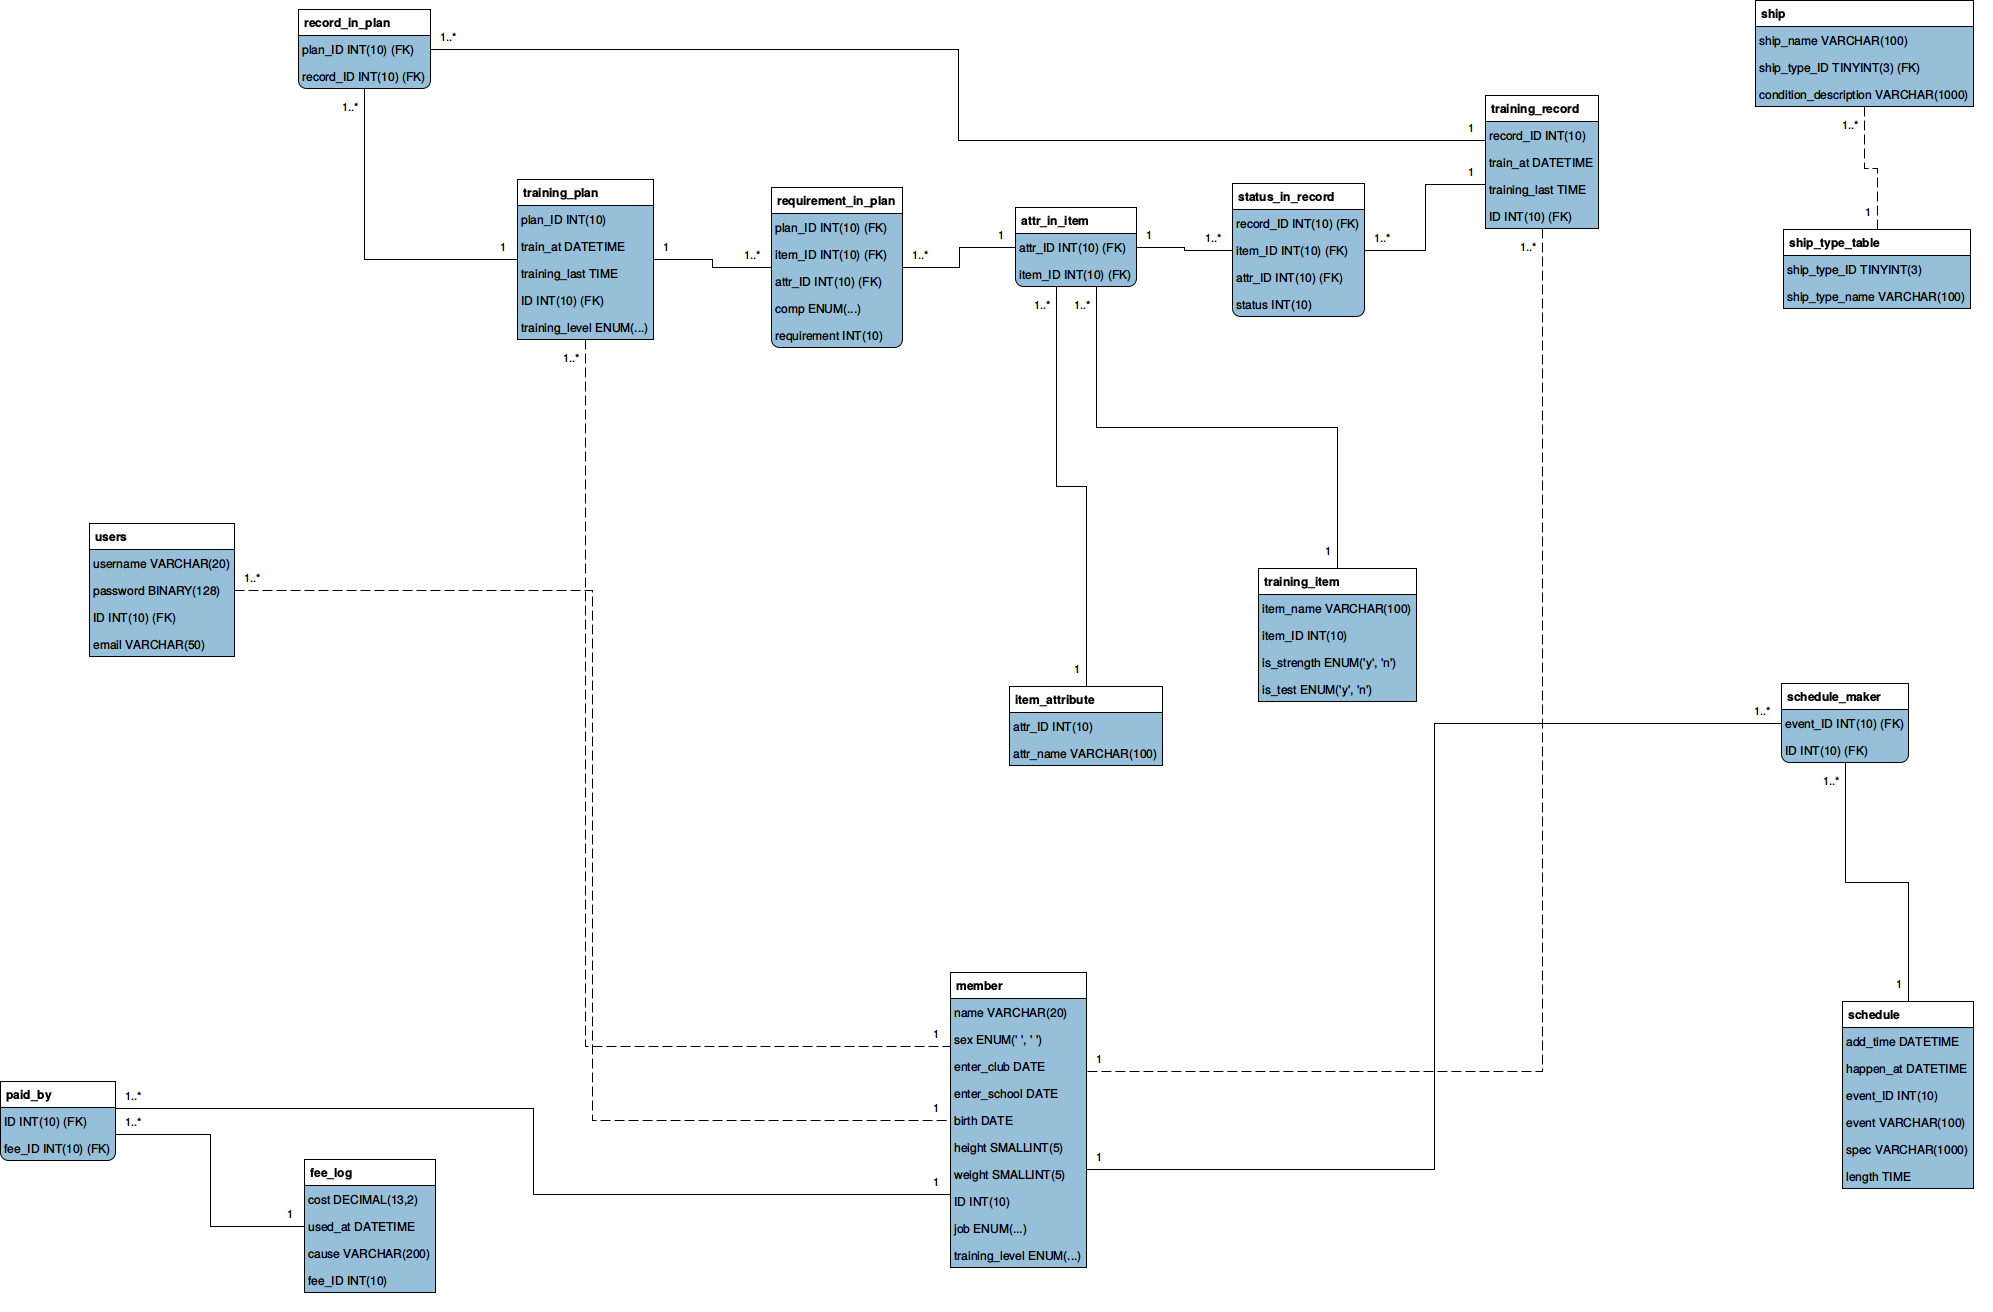
\includegraphics[width=\textwidth]{figure/relation-schema}
\subsection{系统功能模块图}
\tikzstyle{block}=[rectangle,draw=black,fill=white,text centered, anchor=north,
minimum width=3cm]

\tikzstyle{myarray}=[->,>=open triangle 90, thick]

\begin{center}
  \scalebox{.75} {
    \begin{tikzpicture}[node distance=5cm]

      \node(main) [block, xshift=-5cm]{艇员管理系统};

      \node(user) [block, above right of=main, xshift=2cm]{系统管理};
      % ========================================
      \node(login) [block, above right of=user, xshift=2cm, yshift=-2cm]{用户登录};
      \node(logout) [block, below of=login, yshift=4cm]{用户登出};
      \node(password) [block, below of=logout, yshift=4cm]{密码修改};
      \node(user-info) [block, below of=password, yshift=4cm]{修改信息};

      \node(info) [block, below of= user, yshift=0cm]{信息管理};
      % ========================================  
      \node(crew-member) [block, above right of=info, xshift=2cm, yshift=-1cm]{艇员信息管理};
      \node(plan) [block, below of=crew-member, yshift=4cm]{训练计划管理};
      \node(record) [block, below of=plan, yshift=4cm]{训练记录管理};
      \node(ship) [block, below of=record, yshift=4cm]{艇支信息管理};
      \node(fee) [block, below of=ship, yshift=4cm]{支出管理};

      \node(query) [block, below of= info] {信息查询};
      % ========================================
      \node(crew-member-query) [block, above right of=query, xshift=2cm, yshift=-2cm]{艇员信息查询};
      \node(plan-query) [block, below of=crew-member-query, yshift=4cm]{训练计划查询};
      \node(record-query) [block, below of=plan-query, yshift=4cm]{训练记录查询};
      \node(ship-query) [block, below of=record-query, yshift=4cm]{艇支信息查询};
      \node(fee-query) [block, below of=ship-query, yshift=4cm]{支出查询};

      \draw[myarray] (main) |- (user);
      \draw[myarray] (main) |- (info);
      \draw[myarray] (main) |- (query);

      \draw[myarray] (user) |- (login);
      \draw[myarray] (user) |- (logout);
      \draw[myarray] (user) |- (password);
      \draw[myarray] (user) |- (user-info);
      
      \draw[myarray] (info) |- (crew-member);
      \draw[myarray] (info) |- (plan);
      \draw[myarray] (info) |- (record);
      \draw[myarray] (info) |- (ship);
      \draw[myarray] (info) |- (fee);

      \draw[myarray] (query) |- (crew-member-query);
      \draw[myarray] (query) |- (plan-query);
      \draw[myarray] (query) |- (record-query);
      \draw[myarray] (query) |- (ship-query);
      \draw[myarray] (query) |- (fee-query);

      
      
      
      

    \end{tikzpicture}

  }
\end{center}

\subsection{物理结构设计}
\begin{Verbatim}[]
-- with debug if and if not
drop database if exists crewmen;
create database crewmen character set utf8 collate utf8_general_ci;
use crewmen;

drop table if exists users;

drop table if exists schedule_maker;
drop table if exists paid_by;
drop table if exists schedule;
drop table if exists fee_log;

drop table if exists record_in_plan;
drop table if exists requirement_in_plan;
drop table if exists status_in_record;

drop table if exists attr_in_item; -- referenced by requirement and status

drop table if exists training_record; -- by status by record_in_plan
drop table if exists training_plan; -- by requirment by record_in_plan
drop table if exists item_attribute; -- referenced by attr_in_item
drop table if exists training_item; -- referenced by attr_in_item
drop table if exists member; -- referenced by item plan record paid_by schedule_maker users
drop table if exists ship;
drop table if exists ship_type_table;


create table if not exists member
       (name varchar(20) not null,
       -- big chunk for information
       sex enum('男', '女') default '男',
       enter_club date, -- the crew
       enter_school date, -- school
       birth date,
       height smallint unsigned,
       weight smallint unsigned,
       ID int unsigned,
       -- big chunk for information
       job enum('couch', 'crew leader', 'crew member') default 'crew member',
       training_level enum('newbie', 'medium', 'old bird') default 'newbie',
       primary key(ID)
       );-- character set utf8 collate utf8_general_ci;

create table if not exists users
       (username varchar(20) not null,
       password binary(128) not null, -- half byte each, so 128 * 0.5 * 8 is 512 using sha2('pass', 512)
       -- priority tinyint unsigned not null defalut 2, -- the lower the better
       ID int unsigned, -- don't have to be unique, since it's PK for member
       email varchar(50) not null unique,
       primary key(username),
       foreign key(ID) references member(ID) on delete cascade
       );

-- how to enforce constraint on full participation, every schedule should have at least a maker...
create table if not exists schedule
       (add_time datetime default current_timestamp,
       happen_at datetime, -- time could be unsure of
       event_ID int unsigned auto_increment,
       event varchar(100) not null,
       spec varchar(1000),
       length time,
       primary key(event_ID)
       );

create table if not exists schedule_maker
       (event_ID int unsigned,
       ID int unsigned,
       primary key(event_ID, ID),
       foreign key(event_ID) references schedule(event_ID),
       foreign key(ID) references member(ID) on delete cascade
       );


-- same question as schedule, every fee should have a payer
create table if not exists fee_log
       (cost decimal(13,2), -- cost could range from cent to 10^13 which is 10^4 billion yuan, should be enough
        used_at datetime,
        cause varchar(200),
        fee_ID int unsigned,
        primary key(fee_ID)
       );

create table if not exists paid_by
       (ID int unsigned,
       fee_ID int unsigned,
       primary key(ID, fee_ID),
       foreign key(ID) references member(ID) on delete cascade,
       foreign key(fee_ID) references fee_log(fee_ID)
       );

-- plan and record session!!!!!!!!!!!!!!!!!!!!!!!!!!!!!!!!!!!!!!!!!!!!!!!!!!!!!!!!!!!!!!!!!!
-- plan and record session!!!!!!!!!!!!!!!!!!!!!!!!!!!!!!!!!!!!!!!!!!!!!!!!!!!!!!!!!!!!!!!!!!
-- plan and record session!!!!!!!!!!!!!!!!!!!!!!!!!!!!!!!!!!!!!!!!!!!!!!!!!!!!!!!!!!!!!!!!!!
-- plan and record session!!!!!!!!!!!!!!!!!!!!!!!!!!!!!!!!!!!!!!!!!!!!!!!!!!!!!!!!!!!!!!!!!!

-- It's divided into three main parts:
-- The plan and record are symmetrical
-- ignore! no longer supported (although plan can have multiple makes?? weird functionality though)


-- The main similarity lies in the relation of (record, item, attribute, status/requirement)
-- when it indicates that a record can have multiple items
-- when an item can have multiple attributes
-- Therefore this relation can be able to indicate a collection of status of a collection of training items in a plan or record

-- notice how attr_in_item is referenced by (requirement_in_plan and status_in_record)
-- may need to define training item
create table if not exists training_item
       (item_name varchar(100),
       item_ID int unsigned auto_increment,
       is_strength enum('y', 'n'), -- strength or aerobic
       is_test enum('y', 'n'),     -- test or regular
       primary key(item_ID)
       );

create table if not exists training_record
       (record_ID int unsigned auto_increment,
       train_at datetime,
       training_last time,
       ID int unsigned,
       primary key(record_ID),
       foreign key(ID) references member(ID)
       );

create table if not exists training_plan
       (
       plan_ID int unsigned auto_increment,
       train_at datetime,
       training_last time,
       ID int unsigned,
       training_level enum('newbie', 'medium', 'old bird', 'all') default 'all',
       primary key(plan_ID),
       foreign key(ID) references member(ID)
       );

create table if not exists item_attribute
       (attr_ID int unsigned,
       attr_name varchar(100) unique,
       primary key(attr_ID)
       );

create table if not exists attr_in_item
       (attr_ID int unsigned,
       item_ID int unsigned,
       primary key(attr_ID, item_ID),
       foreign key(attr_ID) references item_attribute(attr_ID),
       foreign key(item_ID) references training_item(item_ID)
       );

create table if not exists requirement_in_plan
       (
       plan_ID int unsigned,
       item_ID int unsigned,
       attr_ID int unsigned,
       comp enum('larger', 'smaller', 'no requirement') not null default 'no requirement',
       requirement int unsigned,
       primary key(plan_ID, item_ID, attr_ID),
       foreign key(item_ID, attr_ID) references attr_in_item(item_ID, attr_ID),
       foreign key(plan_ID) references training_plan(plan_ID)
       );

create table if not exists status_in_record
       (record_ID int unsigned,
       item_ID int unsigned,
       attr_ID int unsigned,
       status int unsigned,
       primary key(record_ID, item_ID, attr_ID),
       foreign key (item_ID, attr_ID) references attr_in_item(item_ID, attr_ID),
       foreign key (record_ID) references training_record(record_ID)
       );

-- below is record and plan relation
create table if not exists record_in_plan
       (plan_ID int unsigned,
       record_ID int unsigned,
       primary key(plan_ID, record_ID),
       foreign key(plan_ID) references training_plan(plan_ID),
       foreign key(record_ID) references training_record(record_ID)
       );

-- Obsoleted
-- create table if not exists plan_maker
--        (ID int unsigned,
--        plan_ID int unsigned,
--        primary key(ID, plan_ID),
--        foreign key(ID) references member(ID) on delete cascade,
--        foreign key(plan_ID) references training_plan(plan_ID)
--        );

-- plan and record session!!!!!!!!!!!!!!!!!!!!!!!!!!!!!!!!!!!!!!!!!!!!!!!!!!!!!!!!!!!!!!!!!!
-- plan and record session!!!!!!!!!!!!!!!!!!!!!!!!!!!!!!!!!!!!!!!!!!!!!!!!!!!!!!!!!!!!!!!!!!
-- plan and record session!!!!!!!!!!!!!!!!!!!!!!!!!!!!!!!!!!!!!!!!!!!!!!!!!!!!!!!!!!!!!!!!!!
-- plan and record session!!!!!!!!!!!!!!!!!!!!!!!!!!!!!!!!!!!!!!!!!!!!!!!!!!!!!!!!!!!!!!!!!!

create table if not exists ship_type_table
       (ship_type_ID tinyint unsigned,
       ship_type_name varchar(100),
       primary key(ship_type_ID)
       );

create table if not exists ship
       (ship_name varchar(100),
       ship_type_ID tinyint unsigned,
       condition_description varchar(1000),
       primary key(ship_name),
       foreign key(ship_type_ID) references ship_type_table(ship_type_ID)
       );
\end{Verbatim}

\section{系统功能的实现}
具体实现是利用\textbf{python-flask}框架,以及mysql数据库。

这个项目最主要的模块我认为是训练计划和训练记录,还有用户权限的实现。

\subsection{用户系统}
\paragraph{用户登录}
提供用户名和密码的表单。数据库储存密码这个设计利用的是sha-512的单向hash方式储存。
以后估计会改用bcrypt。因此每次收到密码,在后端要把字符串用hash得到对应的编码与数
据库相应的用户名的密码进行比对。如果正确,从数据库中的成员(member)信息读出权限,
并存放到session里面,并把用户的登录状态还有用户名存放到session里面。

\vspace{3em}
以下是主要的代码:
\begin{Verbatim}[]

\end{Verbatim}

\vspace{3em}
\paragraph{特权机制}
对于某些页面进行限制,比如添加新成员,添加修改训练计划等。如果用户访问受限制的
url,先从登录后存放的session中找到对应的权限。如果权限不足,返回重定向,如果权限
足够,返回对应的页面。

\vspace{3em}
一下是主要的代码:
\begin{Verbatim}[]

\end{Verbatim}

\subsection{训练计划}
\paragraph{计划查询}
每个人都能访问今日的训练计划。

\paragraph{更改计划}
只有队长或者教练能够修改,添加或者删除训练计划。对于返回的表单进行检查。

\subsection{训练记录}

\section{课程设计心得体会}
% \begin{tabular}{p{2cm}|p{8cm}}
% \hline\hline

% \textbf{术语缩写} & \textbf{解释} \\
% \hline\hline

% 术语缩写 & 解释 \\
% \hline

% 术语缩写 & 解释 \\
% \hline

% 术语缩写 & 解释 \\
% \hline

% \hline\hline
% \end{tabular}
% \caption{本文档中出现的术语缩写及解释}
% \end{table}
